\newcommand{\chapter}[2][]{
	\newcommand{\chapname}{#2}
	\begin{flushleft}
		\begin{minipage}[t]{\linewidth}
			
\includegraphics[height=1cm]{hdht-logo.png}
			\hspace{0pt}	
			\sffamily\bfseries\large Bài  12.
			\begin{flushleft}
				\LARGE\bfseries #1
			\end{flushleft}
		\end{minipage}
	\end{flushleft}
	\vspace{1cm}
	\normalfont\normalsize
}
\chapter[Chuyển động của vật bị ném]{Chuyển động của vật bị ném}
\section{Lý thuyết}
\subsection{Chuyển động ném ngang}
Chuyển động ném ngang có thể phân tích thành hai chuyển động thành phần theo hai trục tọa độ (gốc O tại vị trí ném, trục O$x$ hướng theo vectơ vận tốc đầu, trục O$y$ hướng theo vectơ trọng lực).
	\begin{center}
	\begin{tikzpicture}[scale=1, transform shape]  %horizontal projection
		%variable definitions
		\def\g{-9.8} %gravity
		\def\v{10} %velocity
		\def\ang{51} %angle
		\def\s{0.125}
		\pgfmathsetmacro{\c}{{(-1*(2/\g)*\v*sin(\ang))/2}}
		\pgfmathsetmacro{\a}{{(-1*(2/\g)*\v*sin(\ang))*.9}}
		
		\begin{axis}[
			width=.6\linewidth, %set bigger width
			height=3in,
			xmin={{\v*cos(\ang)*\c}},xmax=10, %{\v*cos(\ang)*\a+\s*\v*cos(\ang)}
			ymin=0,ymax={\v*\c*sin(\ang)+0.5*\g*(\c^2)},
			axis x line = top,
			every axis y label/.style={at={(axis description cs:0,-0.05)}},
			every axis x label/.style={at={(axis description cs:1.05,1)},anchor=west},
			xlabel=$x$,
			ylabel=$y$,
			axis y line = left,
			y axis line style={<-},
			x axis line style={<->},
			ticks = none,clip=false,
			]
			
			\tikzset{every mark/.append style={fill=red}}
			
			%flight path
			\addplot[
			dashed,
			domain={\v*cos(\ang)*\c}:10,
			samples=100,]
			{{\g*(x^2)/(2*\v^2*cos(\ang)^2)+x*tan(\ang)}};
			
			%vector at end
			\pgfmathsetmacro{\a}{{(-1*(2/\g)*\v*sin(\ang))*.9}}
			\coordinate (E) at (axis cs:{\v*cos(\ang)*\a},{\v*\a*sin(\ang)+0.5*\g*(\a^2)}){};
			\coordinate (F) at (axis cs:{\v*cos(\ang)*\a+\s*\v*cos(\ang))}, {\v*\a*sin(\ang)+0.5*\g*\a^2+\s*(\v*sin(\ang)+\g*\a)});
			\draw[thick,->](E)--(F);
%			node[midway,sloped,above]{$\vec{V}$};
			\draw[densely dashed,thick,->](E)--(F |- E);
%			node[midway,above]{$\vec{V}_x$};
			\draw[densely dashed,thick,->](E)--(F-| E);
%			node[midway,left]{$\vec{V}_y$};
			
			\path plot[mark=*] coordinates {(E)};
			
			%vector at start
			\pgfmathsetmacro{\c}{{(-1*(2/\g)*\v*sin(\ang))/2}}
			\coordinate (L) at (axis cs:{\v*cos(\ang)*\c},{\v*\c*sin(\ang)+0.5*\g*(\c^2)});
			\coordinate (M) at (axis cs:{\v*cos(\ang)*\c+\s*\v*cos(\ang))},{\v*\c*sin(\ang)+0.5*\g*\c^2+\s*(\v*sin(\ang)+\g*\c)});
			\draw[thick,->](L)--(M)
			node[near end,sloped,above]{$\vec{v}_0$};
			
			\path plot[mark=*] coordinates {(L)};
			
			%vector 1/2 down
			\pgfmathsetmacro{\d}{{(-1*(2/\g)*\v*sin(\ang))*0.6}}
			\coordinate (P) at (axis cs:{\v*cos(\ang)*\d},{\v*\d*sin(\ang)+0.5*\g*(\d^2)});
			\coordinate (Q) at (axis cs:{(\v*cos(\ang)*\d+\s*\v*cos(\ang))},{\v*\d*sin(\ang)+0.5*\g*\d^2+\s*(\v*sin(\ang)+\g*\d)});
			\draw[thick,->](P)--(Q)
			%node[midway,sloped,above]{$\vec{V}$}
			;
			\draw[densely dashed,thick,->](P)--(Q|-P);
%			node[midway,above]{$\vec{V}_x$};
			\draw[densely dashed,thick,->](P)--(Q-|P);
%			node[midway,left]{$\vec{V}_y$};
			
			\path plot[mark=*] coordinates {(P)};
			
			%vector 3/4 down
			\pgfmathsetmacro{\f}{{(-1*(2/\g)*\v*sin(\ang))*0.7}}
			\coordinate (R) at (axis cs:{\v*cos(\ang)*\f},{\v*\f*sin(\ang)+0.5*\g*(\f^2)});
			\coordinate (S) at (axis cs:{(\v*cos(\ang)*\f+\s*\v*cos(\ang))},{\v*\f*sin(\ang)+0.5*\g*\f^2+\s*(\v*sin(\ang)+\g*\f)});
			\draw[thick,->](R)--(S);
%			node[near end,above]{$\vec{v}$};
			\draw[densely dashed,thick,->](R)--(S|-R);
%			node[near end,above,]{$\vec{v}_x$};
			\draw[densely dashed,thick,->](R)--(S-|R);
%			node[near end,left]{$\vec{v}_y$};
			
			\path plot[mark=*] coordinates {(R)};
			
			%vector 1/4 down
			\pgfmathsetmacro{\e}{{(-1*(2/\g)*\v*sin(\ang))*0.8}}
			\coordinate (T) at (axis cs:{\v*cos(\ang)*\e},{\v*\e*sin(\ang)+0.5*\g*(\e^2)});
			\coordinate (U) at (axis cs:{(\v*cos(\ang)*\e+\s*\v*cos(\ang))},{\v*\e*sin(\ang)+0.5*\g*\e^2+\s*(\v*sin(\ang)+\g*\e)});
			\draw[thick,->,blue](T)--(U)
			node[near end,right=2mm]{$\vec{v}$};
			\draw[densely dashed,thick,->,blue](T)--(U|-T)
			node[near end,above]{$\vec{v}_x$};
			\draw[densely dashed,thick,->,blue](T)--(U-|T)
			node[near end,left]{$\vec{v}_y$};
			
			\path plot[mark=*] coordinates {(T)};
		\end{axis}
	\end{tikzpicture}

%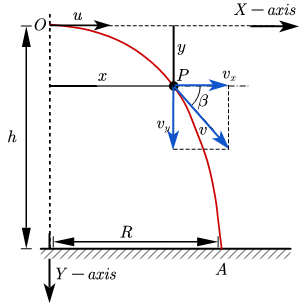
\includegraphics[scale=0.8]{../figs/G10-10-1}
\end{center}

% Hung comment: xóa hình vì không mô tả đúng và không phù hợp, vẫn còn chữ mô tả tiếng Anh trong hình.

\subsubsection{Tính chất của các chuyển động thành phần trên các trục}
	\begin{itemize}
		\item Chuyển động thành phần theo trục O$x$ là chuyển động thẳng đều
			\begin{align*}
				a_x&=0,\\
				v_x&=v_0,\\
				x&=v_xt=v_0t.
			\end{align*}
		\item Chuyển động thành phần theo trục O$y$ là chuyển động rơi tự do không vận tốc đầu
			\begin{align*}
				a_y&=g,\\
				v_y&=0,\\
				y&=\dfrac{1}{2}gt^{2}.
			\end{align*}
	\end{itemize}

%Biết hai chuyển động thành phần, ta suy ra được chuyển động của vật.
\subsubsection{Quỹ đạo của chuyển động ném ngang}
	Phương trình quỹ đạo có thể suy ra bằng cách kết hợp hai phương trình chuyển động trên hai trục $x$ và $y$ 
	\begin{equation*}
		y=\dfrac{g}{2v_0^2}x^2.
	\end{equation*}
	 Quỹ đạo của vật ném ngang có dạng một nửa parabol, đỉnh tại vị trí ném.

\subsubsection{Thời gian chuyển động}
Bằng thời gian rơi tự do của vật được thả từ cùng độ cao:
\begin{equation*}
	t=\sqrt{\dfrac{2h}{g}}.
\end{equation*}
\subsubsection{Tầm ném xa}
Là khoảng cách xa nhất vật đi được theo phương O$x$:
\begin{equation*}
	L = x_{\text{max}} = v_0 t = v_0 \sqrt{\dfrac{2h}{g}}.
\end{equation*}
\subsubsection{Vận tốc của vật khi chạm đất}
Là vận tốc của vật ngay trước khi chạm đất:
\begin{equation*}
	v=\sqrt{v^2_{\text{x}} + v^2_{\text{y}} } = \sqrt{v^2_0+ (gt)^2}.
\end{equation*}
\subsection{Chuyển động ném xiên}
Một chuyển động ném xiên cũng có thể  được phân tích thành hai thành phần: chuyển động thành phần theo phương thẳng đứng và chuyển động thành phần theo phương nằm ngang.
	\begin{center}
	\begin{tikzpicture}[scale=1, transform shape]  %projectile motion
		\begin{axis}[
			width=10cm, %set bigger width
			height=5cm,
			xmin=0,xmax=11.5,
			ymin=0,ymax=4,
			xlabel=$x$,
			ylabel=$y$,
			axis x line = bottom,
			axis y line = left,
			axis line style={->},
			every axis y label/.style={at={(axis description cs:0,1.05)},anchor=south},
			every axis x label/.style={at={(axis description cs:1.02,0)},anchor=west},
			ticks = none,clip=false,
			]
			
			\tikzset{every mark/.append style={fill=red}}
			
			%variable definitions
			\def\g{-9.8} %gravity
			\def\v{10} %velocity
			\def\ang{51} %angle
			\def\s{0.2}
			\pgfmathsetmacro{\t}{0}
			%flight path
			\addplot[
			dashed,
			domain=0:10,
			samples=100,]
			{{\g*(x^2)/(2*\v^2*cos(\ang)^2)+x*tan(\ang)}};
%			node[midway,above]{$V_y=0$};
			
			%vector at start
			\coordinate (A) at (axis cs: {\v*cos(\ang)*\t}, {\v*\t*sin(\ang)+0.5*\g*(\t^2)});
			\coordinate (B) at (axis cs: {\v*cos(\ang)*\t+\s*\v*cos(\ang)}, {\v*\t*sin(\ang)+0.5*\g*\t^2+\s*(\v*sin(\ang)+\g*\t)});
			\draw[thick,->](A)--(B)
			node[near end,above right=3mm and 0.5mm]{$\vec{v}_0$};
			\draw[densely dashed,thick,->](A)--(B|-A)
			node[near end,below]{$\vec{v}_{0x}$};
			\draw[densely dashed,thick,->](A)--(B-|A)
			node[near end,left]{$\vec{v}_{0y}$};
			
			\path plot[mark=*] coordinates {(A)};
			
			%dashed box around start vector
			\draw[dashed](B-|A)--(B);
			\draw[dashed](B|-A)--(B);
			
			%vector at end
			\pgfmathsetmacro{\a}{{-1*(2/\g)*\v*sin(\ang)}}
			\coordinate (E) at (axis cs:{\v*cos(\ang)*\a},{\v*\a*sin(\ang)+0.5*\g*(\a^2)}){};
%			\coordinate (F) at (axis cs:{\v*cos(\ang)*\a+\s*\v*cos(\ang))}, {\v*\a*sin(\ang)+0.5*\g*\a^2+\s*(\v*sin(\ang)+\g*\a)});
%			\draw[very thick,->](E)--(F)
%			node[midway,sloped,above]{$V$};
%			\draw[densely dashed,very thick,->](E)--(F |- E)
%			node[midway,above]{$V_x$};
%			\draw[densely dashed,very thick,->](E)--(F-| E)
%			node[midway,left]{$V_y$};
			
%			\path plot[mark=*] coordinates {(E)};
			
			%vector 1/2 up
			\pgfmathsetmacro{\b}{{(-1*(2/\g)*\v*sin(\ang))/4}}
			\coordinate (H) at (axis cs:{\v*cos(\ang)*\b},{\v*\b*sin(\ang)+0.5*\g*(\b^2)});
			\coordinate (I) at (axis cs: {\v*cos(\ang)*\b+\s*\v*cos(\ang)},{\v*\b*sin(\ang)+0.5*\g*\b^2+\s*(\v*sin(\ang)+\g*\b)});
			\draw[thick,->](H)--(I);
%			node[midway,sloped,above]{$V$};
			\draw[densely dashed,thick,->](H)--(I-|H);
%			node[midway,left]{$V_x$};
			\draw[densely dashed,thick,->](H)--(I|-H);
%			node[midway,below]{$V_y$};
			
			\path plot[mark=*] coordinates {(H)};
			
			%vector halfway
			\pgfmathsetmacro{\c}{{(-1*(2/\g)*\v*sin(\ang))/2}}
			\coordinate (L) at (axis cs:{\v*cos(\ang)*\c},{\v*\c*sin(\ang)+0.5*\g*(\c^2)});
			\coordinate (M) at (axis cs:{\v*cos(\ang)*\c+\s*\v*cos(\ang))},{\v*\c*sin(\ang)+0.5*\g*\c^2+\s*(\v*sin(\ang)+\g*\c)});
			\draw[thick,->](L)--(M);
%			node[near end,sloped,right=2mm]{$\vec{v}$};
			
			
			%T2 line; halfway up flight path
			\draw[loosely dashed,] (L) -- (axis cs:{\v*cos(\ang)*\c},0)
			node[midway,right] {$H$};
			
			
			\path plot[mark=*] coordinates {(L)};
			
			%vector 1/2 down
			\pgfmathsetmacro{\d}{{(-1*(2/\g)*\v*sin(\ang))*0.75}}
			\coordinate (P) at (axis cs:{\v*cos(\ang)*\d},{\v*\d*sin(\ang)+0.5*\g*(\d^2)});
			\coordinate (Q) at (axis cs:{(\v*cos(\ang)*\d+\s*\v*cos(\ang))},{\v*\d*sin(\ang)+0.5*\g*\d^2+\s*(\v*sin(\ang)+\g*\d)});
			\draw[thick,->](P)--(Q);
%			node[midway,sloped,below]{$V$};
			\draw[densely dashed,thick,->](P)--(Q|-P);
%			node[midway,above]{$V_x$};
			\draw[densely dashed,thick,->](P)--(Q-|P);
%			node[midway,left]{$V_y$};
			
			\path plot[mark=*] coordinates {(P)};
			
			%start vector angle label
			\node[circle,minimum size=25pt] at (A) (circ) {};
			\node[right] at (circ.30) {$\theta$};
			\path[clip] (A) -- (B) -- (B|-A) -- cycle;
			\node[circle,draw,minimum size=25pt] at (A) (circ) {};
			
%			\draw[<->,blue] (A)++(0,1cm) -- (E)++(0,1cm);
		\end{axis}
	\end{tikzpicture}	
%	\begin{tikzpicture}[x=(330:1cm),y=(30:1cm),z=(90:1cm)]
		% green ground
%		\fill [LightGreen] (-1,-1,0) -- (-.5,1,0) -- (11,2,0) -- (11,-2,0) -- cycle;
%		\fill[Green] (9,0,0) circle [x radius=1.5, y radius=1];
		% black hole
%		\fill[black] (10,0,0) circle [x radius=.1, y radius=.1];
		% red flag
%		\draw[Brown, thick, line cap=round] (10,0,0) -- (10,0,1);
%		\fill[Red] (10,0,1) -- (9.8,0,0.9) -- (10,0,0.8) -- cycle;
		% yellow sand hill
%		\fill[Yellow, shift={(7,0,0)}] 
%		plot [domain=0:340, samples=20, smooth cycle, variable=\t] 
%		(\t:rnd/16+0.25 and rnd/8+0.75);
		
		% origin
%		\node[below left] {$O$};
		% x-axis
%		\draw (0, 0) -- (10, 0) 
%		node[midway, yshift=-.8cm, rotate=330] {Distance, x (m)};
%		\draw foreach \i in {2,4,6,8} 
%		{ (\i, 0) node[below, rotate=330] {\i} -- ++(0, .15) };
		% y-axis
%		\draw (0, 0, 0) -- (0, 0, 5) 
%		node[pos=.8, xshift=-.8cm, rotate=90] {Height, y(m)};
%		\draw foreach \i in {2,4} 
%		{ (0, 0, \i) node[left] {\i} -- ++(.15, 0, 0) };
		
%		\foreach \a[evaluate={\v=70; \T=\v*sin(\a)/9.807*2;}] in {60} {
%			\draw[x=(330:0.5pt), z=(90:0.5pt), Black, dashed]
%			plot [smooth, domain=0:\T, samples=50, variable=\t,
%			mark=*, mark repeat=2, mark size=1.8pt, mark options={fill=white, solid}]
%			(\v*\t*cos \a, 0, -9.807/2*\t^2+\v*\t*sin \a +0.1016) coordinate (end);
%			\filldraw[fill=White] (end) circle [radius=1.8pt];
%		}
%	\end{tikzpicture}
\end{center}

%\begin{center}
%	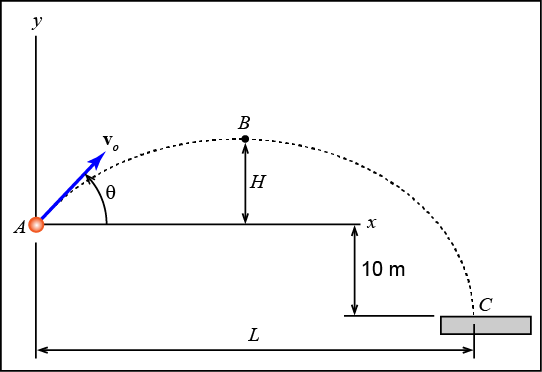
\includegraphics[scale=0.8]{../figs/G10-10-2}
%\end{center}

% Hung comment: hình vẽ G10-10-2 sai, không phù hợp với nội dung. Đã thay thế bằng hình vẽ với tikz pgfplot trên.		

\subsubsection{Tính chất của các chuyển động thành phần trên các trục}
	\begin{itemize}
		\item Chuyển động thành phần theo trục O$x$ là chuyển động thẳng đều 
			\begin{align*}
				a_x&=0,\\
				v_x&=v_{0x}=v_0\cos\theta,\\
				x&=v_xt=v_0\cos\theta t.
			\end{align*}
		\item Chuyển động thành phần theo trục O$y$ là chuyển động rơi tự do có vận tốc đầu
			\begin{align}
				a_y&=-g,\\
				v_y&=v_{0y}-gt=v_0\sin\theta-gt,\\
				y&=v_{0y}t-\dfrac{1}{2}gt^{2}=v_0\sin\theta t-\dfrac{1}{2}gt^{2}.
			\end{align}
	\end{itemize} 
\subsubsection{Độ cao cực đại}
	Khi vật lên đến độ cao cực đại, thành phần vận tốc theo phương $y$ triệt tiêu. 
		\begin{align*}
			H=y_{\max}=\dfrac{v_0^2\sin^2\theta}{2g}
		\end{align*}
	
\subsubsection{Tầm xa}
		\vspace{-0.5cm}
		\begin{align*}
			L = x_{\max} = \dfrac{v_0^2 \sin 2\theta}{g}.
		\end{align*}
	



\section{Mục tiêu bài học - Ví dụ minh họa}
\begin{dang}{Ghi nhớ đặc điểm và công thức \\ của chuyển động ném ngang}
	\viduii{1}{Một vật được ném ngang từ độ cao $h$ so với mặt đất ở nơi có gia tốc rơi tự do $g$. Thời gian chạm đất của vật là
		\begin{mcq}(2)
			\item $t=\sqrt{\dfrac{2h}{g}}.$
			\item $t=\dfrac{2h}{g}.$
			\item $t=\dfrac{h}{2g}$
			\item $t=\sqrt{\dfrac{h}{2g}}$
		\end{mcq}
	}
	{	\begin{center}
			\textbf{Hướng dẫn giải}
		\end{center}
		
		Thời gian chuyển động bằng thời gian rơi tự do của vật được thả từ cùng độ cao
		\begin{equation*}
			t=\sqrt{\dfrac{2h}{g}}.
		\end{equation*}
		
		\textbf{Đáp án: A}.
	}
	\viduii{1}{Ở nơi có gia tốc rơi tự do là $g$, từ độ cao $h$ so với mặt đất, một vật được ném ngang với tốc độ ban đầu $v$. Tầm bay xa của vật là
		\begin{mcq}(2)
			\item $L = v_0 \sqrt{\dfrac{h}{2g}}.$
			\item $L = v_0 \dfrac{2h}{g}.$
			\item $L = v_0 \dfrac{h}{2g}.$
			\item $L = v_0 \sqrt{\dfrac{2h}{g}}.$ 
		\end{mcq}
	}
	{	\begin{center}
			\textbf{Hướng dẫn giải}
		\end{center}
		
		Tầm ném xa
		
		\begin{equation*}
			L = x_{\text{max}} = v_0 t = v_0 \sqrt{\dfrac{2h}{g}}.
		\end{equation*}
		
		\textbf{Đáp án: D}.
	}
\end{dang}
\begin{dang}{Xây dựng phương trình quỹ đạo, \\giải bài toán về chuyển động ném ngang}
	\viduii{3}{Một viên đạn được bắn theo phương ngang ở độ cao $\SI{180}{m}$ phải có vận tốc ban đầu là bao nhiêu để ngay lúc chạm đất có $v = \SI{100}{m/s}$. Tính tầm ném xa của vật khi chạm đất.
	}
	{	\begin{center}
			\textbf{Hướng dẫn giải}
		\end{center}
		
		Thời gian chuyển động
			\begin{equation*}
				t=\sqrt{\dfrac{2h}{g}} = \SI{6}{s}
			\end{equation*}
		Vận tốc ban đầu 
			\begin{equation*}
				v^2 = v^2_{\text{x}} + v^2_{\text{y}}  = v^2_0+ (gt)^2 \Rightarrow v_0 =\sqrt{ v^2 -(gt)^2} = \SI{80}{m/s}.  
			\end{equation*}
		Tầm ném xa của vật khi chạm đất
			\begin{equation*}
				L=v_0 t  = \SI{480}{m}.
			\end{equation*}

	}
	\viduii{3}{Từ sân thượng cao $\SI{20}{m}$ một người đã ném  một hòn sỏi theo phương ngang với $v_0 = \SI{4}{m/s}$, $g = \SI{10}{m/s^2}$.
		\begin{enumerate}[label=\alph*.]
			\item Viết phương trình chuyển động của hòn sỏi theo trục $Ox$, $Oy$.
			\item Viết phương trình quỹ đạo của hòn sỏi.
			\item Hòn sỏi đạt tầm xa bằng bao nhiêu? Vận tốc của nó khi vừa chạm đất.
		\end{enumerate}
		}
	{	\begin{center}
			\textbf{Hướng dẫn giải}
		\end{center}
		\begin{enumerate}[label=\alph*.]
			\item Chọn gốc tọa độ O ở sân thượng. Trục $Ox$ thẳng đứng hướng xuống. Gốc thời gian là lúc ném hòn sỏi. Phương trình chuyển động của hòn sỏi
			\begin{equation*}
				\begin{cases}
					x =v_0t = 4t. \\
					y = \dfrac{1}{2}gt^2 =5t^2.
				\end{cases}
			\end{equation*}
			\item Phương trình quỹ đạo của hòn sỏi thu được bằng cách kết hợp hai phương trình chuyển động thành phần trên hai trục
				\begin{align*}
					x&=v_0t	\quad\Rightarrow\quad t=\dfrac{x}{v_0}\\
					y&=\dfrac{1}{2}gt^{2}=\dfrac{1}{2}g\left(\dfrac{x}{v_0}\right)^{2}= \dfrac{5}{16}x^2.
				\end{align*}
			\item Khi rơi chạm đất $y = \SI{20}{cm}$
				$$y=\dfrac{5}{16}x^2 =20 \quad\Rightarrow\quad x = \SI{8}{m}.$$
			
			Tầm xa của hòn sỏi $L =\SI{8}{m}.$
			
			Thời gian hòn sỏi chạm đất
			
			$$t=\sqrt{\dfrac{2h}{g}} = \SI{2}{s}.$$
			
			Vận tốc của hòn sỏi khi chạm đất 
			
			$$v=\sqrt{v^2_{\text{x}} + v^2_{\text{y}}} = \sqrt{v^2_0+ (gt)^2} = \SI{20,4}{m/s}.$$
		\end{enumerate}
	}
\end{dang}
